\section{Theorie}
\label{sec:Theorie}

Mithilfe der Maxwellschen Gleichungen mit

\begin{equation*}
    \label{eq:maxwell4}
    \nabla \times \vec{H} = \vec{j} + \varepsilon \, \varepsilon_0 \, \dfrac{\dif \vec{E}}{\dif t} 
\end{equation*}
und
\begin{equation*}
    \label{eq:maxwell2}
    \nabla \times \vec{E} = - \mu \, \mu_0 \, \frac{\dif \vec{H}}{\dif t} 
\end{equation*}

lässt sich jeder elektromagnetischen Welle unter Verwendung von

\begin{equation*}
    W_{\text{el}} := \frac{1}{2} \, \varepsilon \, \varepsilon_0 \, \vec{E}^2
\end{equation*}
und
\begin{equation*}
    W_{\text{mag}} := \frac{1}{2} \, \mu_0 \, \vec{H}^2
\end{equation*}
als Ausdrücke der elektrischen bzw. magnetischen Energie pro Volumen eine Strahlungsleistung in Form des Poynting-Vektors zuordnen. 

Im Betrag ergibt sich dieser dann zu
\begin{equation}
    \left| \vec{S} \right|  = v \, \varepsilon \, \varepsilon_0 \, \vec{E}^2 \,.
    \label{eq:betragpoynting}
\end{equation} \\

\newpage

Trifft nun eine ebene Lichtwelle unter dem Winkel $\alpha$ aus dem Vakuum auf eine Grenzfläche zu einem anderen Medium, 
so wird ein Teil der Strahlung mit der Amplitude $\vec{E_r}$ gebrochen, der andere mit der Amplitude $\vec{E_d}$ reflektiert.
Dabei soll angenommen werden, dass dieser Vorgang vollständig absorptionsfrei verläuft, also keine Energie an der Grenzfläche 'verloren' geht.
\begin{figure}[H]
    \centering
    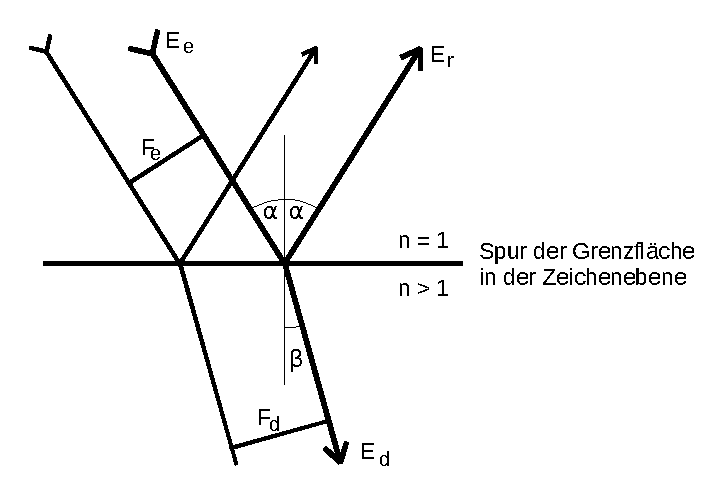
\includegraphics{Brechung an einer Ebene.pdf}
    \caption{Brechung an einer Ebene \cite{ap01}.} 
    \label{fig:abb1}
\end{figure}

Wie in \autoref{fig:abb1} zu erkennen ist, gilt aufgrund der geringen Lichtgeschwindigkeit $v$ im Zweitmedium $\beta < \alpha$, der Brechungswinkel ist also kleiner als der Einfalls- bzw. Reflexionswinkel.
Daraus bedingt sich eine Querschnittsänderung der einlaufenden Strahlung von $F_e$ auf $F_d$. \\

Es gilt die Energieerhaltung, die sich als
\begin{equation*}
    S_{\text{e}} \, F_{\text{e}} = S_{\text{r}} \, F_{\text{e}} +  S_{\text{d}} \, F_{\text{d}}
    \label{eq:Energieerhaltung}
\end{equation*}
oder auch 
\begin{equation}
    S_{\text{e}} \cos(\alpha) = S_{\text{r}} \cos(\alpha) +  S_{\text{d}} \cos(\beta)
    \label{eq:Energieerhaltungwinkel}
\end{equation}
schreiben lässt. \\

Die Gleichung \eqref{eq:Energieerhaltungwinkel} lässt sich mit hilfe der Gleichung \eqref{eq:betragpoynting} für die Poynting-Vektoren zu 
\begin{equation}
    c \, \varepsilon_0 \, \vec{E}^2_{\text{e}} \, \cos(\alpha) = c \, \varepsilon_0 \, \vec{E}^2_{\text{r}} \, \cos(\alpha) + v \, \varepsilon \, \varepsilon_0 \, \vec{E}^2_{\text{d}} \, \cos(\beta)
    \label{eq:eins}
\end{equation}
umstellen.\\

Der Brechungsindex ist das Verhältnis zwischen der Lichtgeschwindigkeit im Vakuum und der im Medium 
\begin{equation*}
    n = \dfrac{\text{c}}{v} ,
    \label{eq:Brechungsindex}
\end{equation*}
damit kann anstelle der Gleichung \eqref{eq:eins} auch
\begin{equation}
    (\vec{E}^2_{\text{e}}  - \vec{E}^2_{\text{r}}) \, n \, \cos(\alpha) = \varepsilon \, \vec{E}^2_{\text{d}} \, \cos(\beta)
    \label{eq:zwei}
\end{equation}
geschrieben werden. \\

Wenn die Maxwellsche Relation
\begin{equation*}
    n^2 = \varepsilon
    \label{eq:Maxwellschrelation}
\end{equation*}
in die Gleichung \eqref{eq:zwei} eingesetzt wird, ergibt sich 
\begin{equation}
    (\vec{E}^2_{\text{e}}  - \vec{E}^2_{\text{r}}) \, \cos(\alpha) = n \, \vec{E}^2_{\text{d}} \, \cos(\beta) \,.
    \label{eq:drei}
\end{equation}

Die eingehende Welle, die durch den Vektor $\vec{E_e}$ gegeben ist, besteht aus einem parallel und senkrecht polarisierten Teil.
\begin{equation*}
    \vec{E_e} = \vec{E_\parallel}  + \vec{E_\perp}
    \label{eq:vier}
\end{equation*}
Die unterschiedlich polarisierten Teile der Welle verhalten sich an der Grenzfläche verschieden.
Aus diesem Grund ist es notwendig den parallelen und senkrechten Teil seperat zu betrachten.\\

\newpage

Zunächst soll hier der senkrecht polarisierte Teil betrachtet werden.
Wie in \autoref{fig:abb2} dargestellt, passiert die Tangentialkomponente des Feldstärkevektors die Grenzfläche stetig, sie ist also auf beiden Seiten gleich.

\begin{figure}[H]
    \centering
    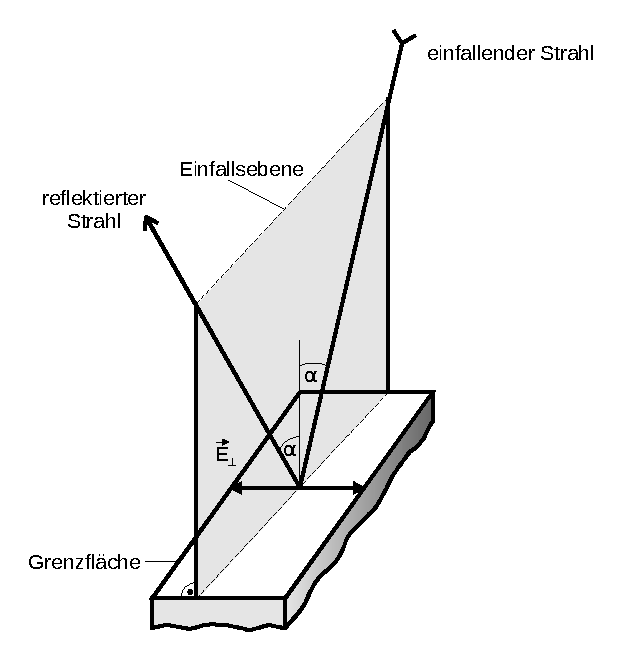
\includegraphics{Brechung mit senkrechter Strahlung.pdf}
    \caption{Reflexion eines senkrecht polarisierten Lichtstrahls \\ an einer Grenzfläche \cite{ap01}.}
    \label{fig:abb2}
\end{figure}

Hier entsprechen die Beträge des senkrechten Strahls den Tangentialkomponenten, es gilt also
\begin{equation}
    \vec{E}_{\text{e}_{\perp}} + \vec{E}_{\text{r}_{\perp}} = \vec{E}_{\text{d}_{\perp}} \,.
    \label{eq:esenkrecht}
\end{equation}

Aus \eqref{eq:drei} lässt sich mithilfe von \eqref{eq:esenkrecht} nun $E_{\text{d}}$ eliminieren, es ergibt sich
\begin{equation}
    \vec{E}_{\text{r}_{\perp}} = - \vec{E}_{\text{e}_{\perp}} \, \frac{n \, \cos(\beta) - \cos(\alpha)}{n \, \cos(\beta) + \cos(\alpha)} \,.
    \label{eq:E_rsenkrecht}
\end{equation}

Unter Betrachtung des Snelliuschen Brechungsgesetzes mit
\begin{equation*}
    n = \frac{\sin(\alpha)}{\sin(\beta)}
    \label{eq:snellius}
\end{equation*}
vereinfacht sich \eqref{eq:E_rsenkrecht} dann entweder zu
\begin{equation*}
    \vec{E}_{\text{r}_{\perp}}(\alpha) = - \vec{E}_{\text{e}_{\perp}} \, \frac{\sin(\alpha - \beta)}{\sin(\alpha + \beta)}
\end{equation*}
oder
\begin{equation}
    \vec{E}_{\text{r}_{\perp}}(\alpha) = - \vec{E}_{\text{e}_{\perp}} \, \frac{\left( \sqrt{n^2 - \sin^2(\alpha)} - \cos^2(\alpha) \right)^2}{n^2 - 1} \,.
    \label{eq:E_rsenkrecht+snell}
\end{equation}

Dabei gilt für $\alpha = \dfrac{\pi}{2}$, also den streifenden Einfall
\begin{equation*}
    \vec{E}_{\text{r}_{\perp}} \left(\frac{\pi}{2} \right) = - \vec{E}_{\text{e}_{\perp}}
\end{equation*}
und für $\alpha = 0$, also den senkrechten Einfall
\begin{equation*}
    \vec{E}_{\text{r}_{\perp}}(0) = - \vec{E}_{\text{e}_{\perp}} \, \frac{n - 1}{n + 1} \,.
\end{equation*} \\

Für parallel polarisiertes Licht folgen nach \autoref{fig:abb3} für die Tangentialkomponenten
\begin{align*}
    \vec{E}_{\text{e}\parallel \text{tg}} = \vec{E}_{\text{e}\parallel} \, \cos(\alpha), && \vec{E}_{\text{r}\parallel \text{tg}} = - \vec{E}_{\text{r}\parallel} \, \cos(\alpha) \, &&
    \text{und} && \vec{E}_{\text{d}\parallel \text{tg}} = \vec{E}_{\text{d}\parallel} \cos(\beta) \,.
\end{align*}

\begin{figure}[H]
    \centering
    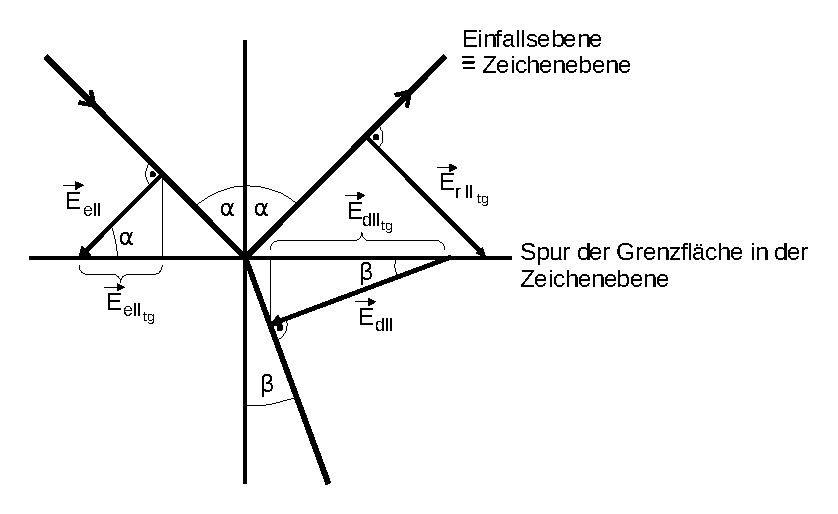
\includegraphics{Brechung mit paralleler Strahlung.pdf}
    \caption{Reflexion eines parallel polarisierten Lichtstrahls \\ an einer Grenzfläche \cite{ap01}.}
    \label{fig:abb3}
\end{figure}

Unter Zuhilfenahme der Stetigkeitsbedingung
\begin{equation*}
    \vec{E}_{\text{e}\parallel \text{tg}} + \vec{E}_{\text{r}\parallel \text{tg}} = \vec{E}_{\text{d}\parallel \text{tg}}
\end{equation*}
bzw.
\begin{equation}
    (\vec{E}_{\text{e}\parallel} - \vec{E}_{\text{r}\parallel}) \, \cos(\alpha) = \vec{E}_{\text{d}\parallel} \cos(\beta)
    \label{eq:stetigkeitsbedEpar}
\end{equation}
ergibt sich \eqref{eq:drei} zu
\begin{equation*}
    \vec{E}_{\text{r}\parallel} = \vec{E}_{\text{e}\parallel} \, \frac{n \, \cos(\alpha) - \cos(\beta)}{n \, \cos(\alpha) + \cos(\beta)}
\end{equation*}
und 
\begin{equation}
    \vec{E}_{\text{r}\parallel} = \vec{E}_{\text{e}\parallel} \, \frac{\tan(\alpha - \beta)}{\tan(\alpha + \beta)}
    \label{eq:E_par}
\end{equation}
oder mithilfe von Snellius zu
\begin{equation}
    \vec{E}_{\text{r}\parallel} (\alpha) = \vec{E}_{\text{e}\parallel} \, \frac{n^2 \, \cos(\alpha - \sqrt{n^2 - \sin^2(\alpha)})}{n^2 \, \cos(\alpha) + \sqrt{n^2 - \sin^2(\alpha)}} \,.
    \label{eq:E_parSnellius}
\end{equation} \\

Auch hier lassen sich erneut die Spezialfälle $\alpha = 0$ und $\alpha = \dfrac{\pi}{2}$ betrachten. Es folgt

\begin{equation*}
    \vec{E}_{\text{r}\parallel}(0) = \vec{E}_{\text{e}\parallel} \, \frac{n - 1}{n + 1}
\end{equation*}
sowie
\begin{equation*}
    \vec{E}_{\text{r}\parallel} \left(\frac{\pi}{2} \right) = - \vec{E}_{\text{e}\parallel} \,.
\end{equation*}\\

Dabei wird nach \eqref{eq:E_par} für $\alpha_p + \beta_p = \dfrac{\pi}{2}$ $\vec{E}_{\text{r}\parallel} (\alpha_p) = 0$, nach Snellius folgt also
\begin{equation*}
    \tan(\alpha_p) = n \,.
    \label{eq:Brewsterwinkel}
\end{equation*}
Der Winkel $\alpha_p$ wird dabei als Brewsterwinkel bezeichnet und beschreibt den Winkel, ab dem kein Licht mehr reflektiert wird, es also vollständig ins Medium eindringt.
